\chapter{Simuleren van gedrag op basis van een sequentiediagram}\label{sec:gedrag}
Een ander populair type van UML-diagram is het sequentiediagram. Waar klassediagrammen de informatie bevat in klasses en de verbanden tussen klasses benoemen, beschrijven sequentiediagrammen het gedrag van instanties van de klasses. Deze instanties communiceren via berichten. Doorgaans zijn deze berichten ofwel een oproep van een methode gedefinieerd voor de klasse van een instantie ofwel een instantiatie van een nieuwe instantie. De berichten zijn genummerd volgens een bepaalde volgorde en samen modelleren ze het gedrag van een stuk van de software.

\parbreak

Figuur \ref{fig:seq-diagram-game} geeft een voorbeeld van een sequentiediagram gebaseerd op het klassediagram voorgesteld in figuur \ref{fig:diagram-voorbeeld}.

Een instantie wordt voorgesteld door een kader met daarin tekst volgens het patroon \textit{instantienaam : klassenaam}. Dit wil zeggen dat bijvoorbeeld \textit{attacker} een instantie is van de klasse \textit{Character}. Vanuit elk kader vertrekt ook een streepjeslijn: de \textbf{levenslijn}. Deze levenslijn kan ingevuld worden door gekleurde balken, welke de duur van een oproep van een methode aan een instantie voorstellen.
Verder zijn er ook kaders die berichten omsluiten. Deze kaders duiden \textbf{gecombineerde fragmenten} aan, en in deze tekst beschouwen we twee soorten:

\begin{enumerate}
	\item Het \textbf{altfragment}: Deze soort duidt een \textit{if-else}-constructie aan. Het bestaat uit twee delen, namelijk het \text{if}-deel en het \textit{else}-deel, en er staat aangeduid onder welke voorwaarden welk deel wordt uitgevoerd. Figuur \ref{fig:seq-diagram-game} bevat een voorbeeld van een altfragment.
	\item Het \textbf{lusfragment}: Deze soort duidt een lusconstructie aan. Er staat aangeduid onder welke voorwaarden er een iteratie wordt uitgevoerd. Deze voorwaarde wordt gecontroleerd zowel v\'o\'or de eerste keer dat er mogelijks een iteratie wordt uitgevoerd als elke keer dat een iteratie ten einde komt. Indien de voorwaarde niet geldt, wordt de lus overgeslagen. \todo{referentie naar figuur met loop fragment}
\end{enumerate}

In dit hoofdstuk beschouwen we hoe we het vocabularium en de logische theorie die we hebben opgebouwd eerder in de tekst kunnen uitbreiden om het gedrag voorgesteld in een sequentiediagram te modelleren.

\begin{landscape}
\begin{figure}
	\label{fig:seq-diagram-game}
	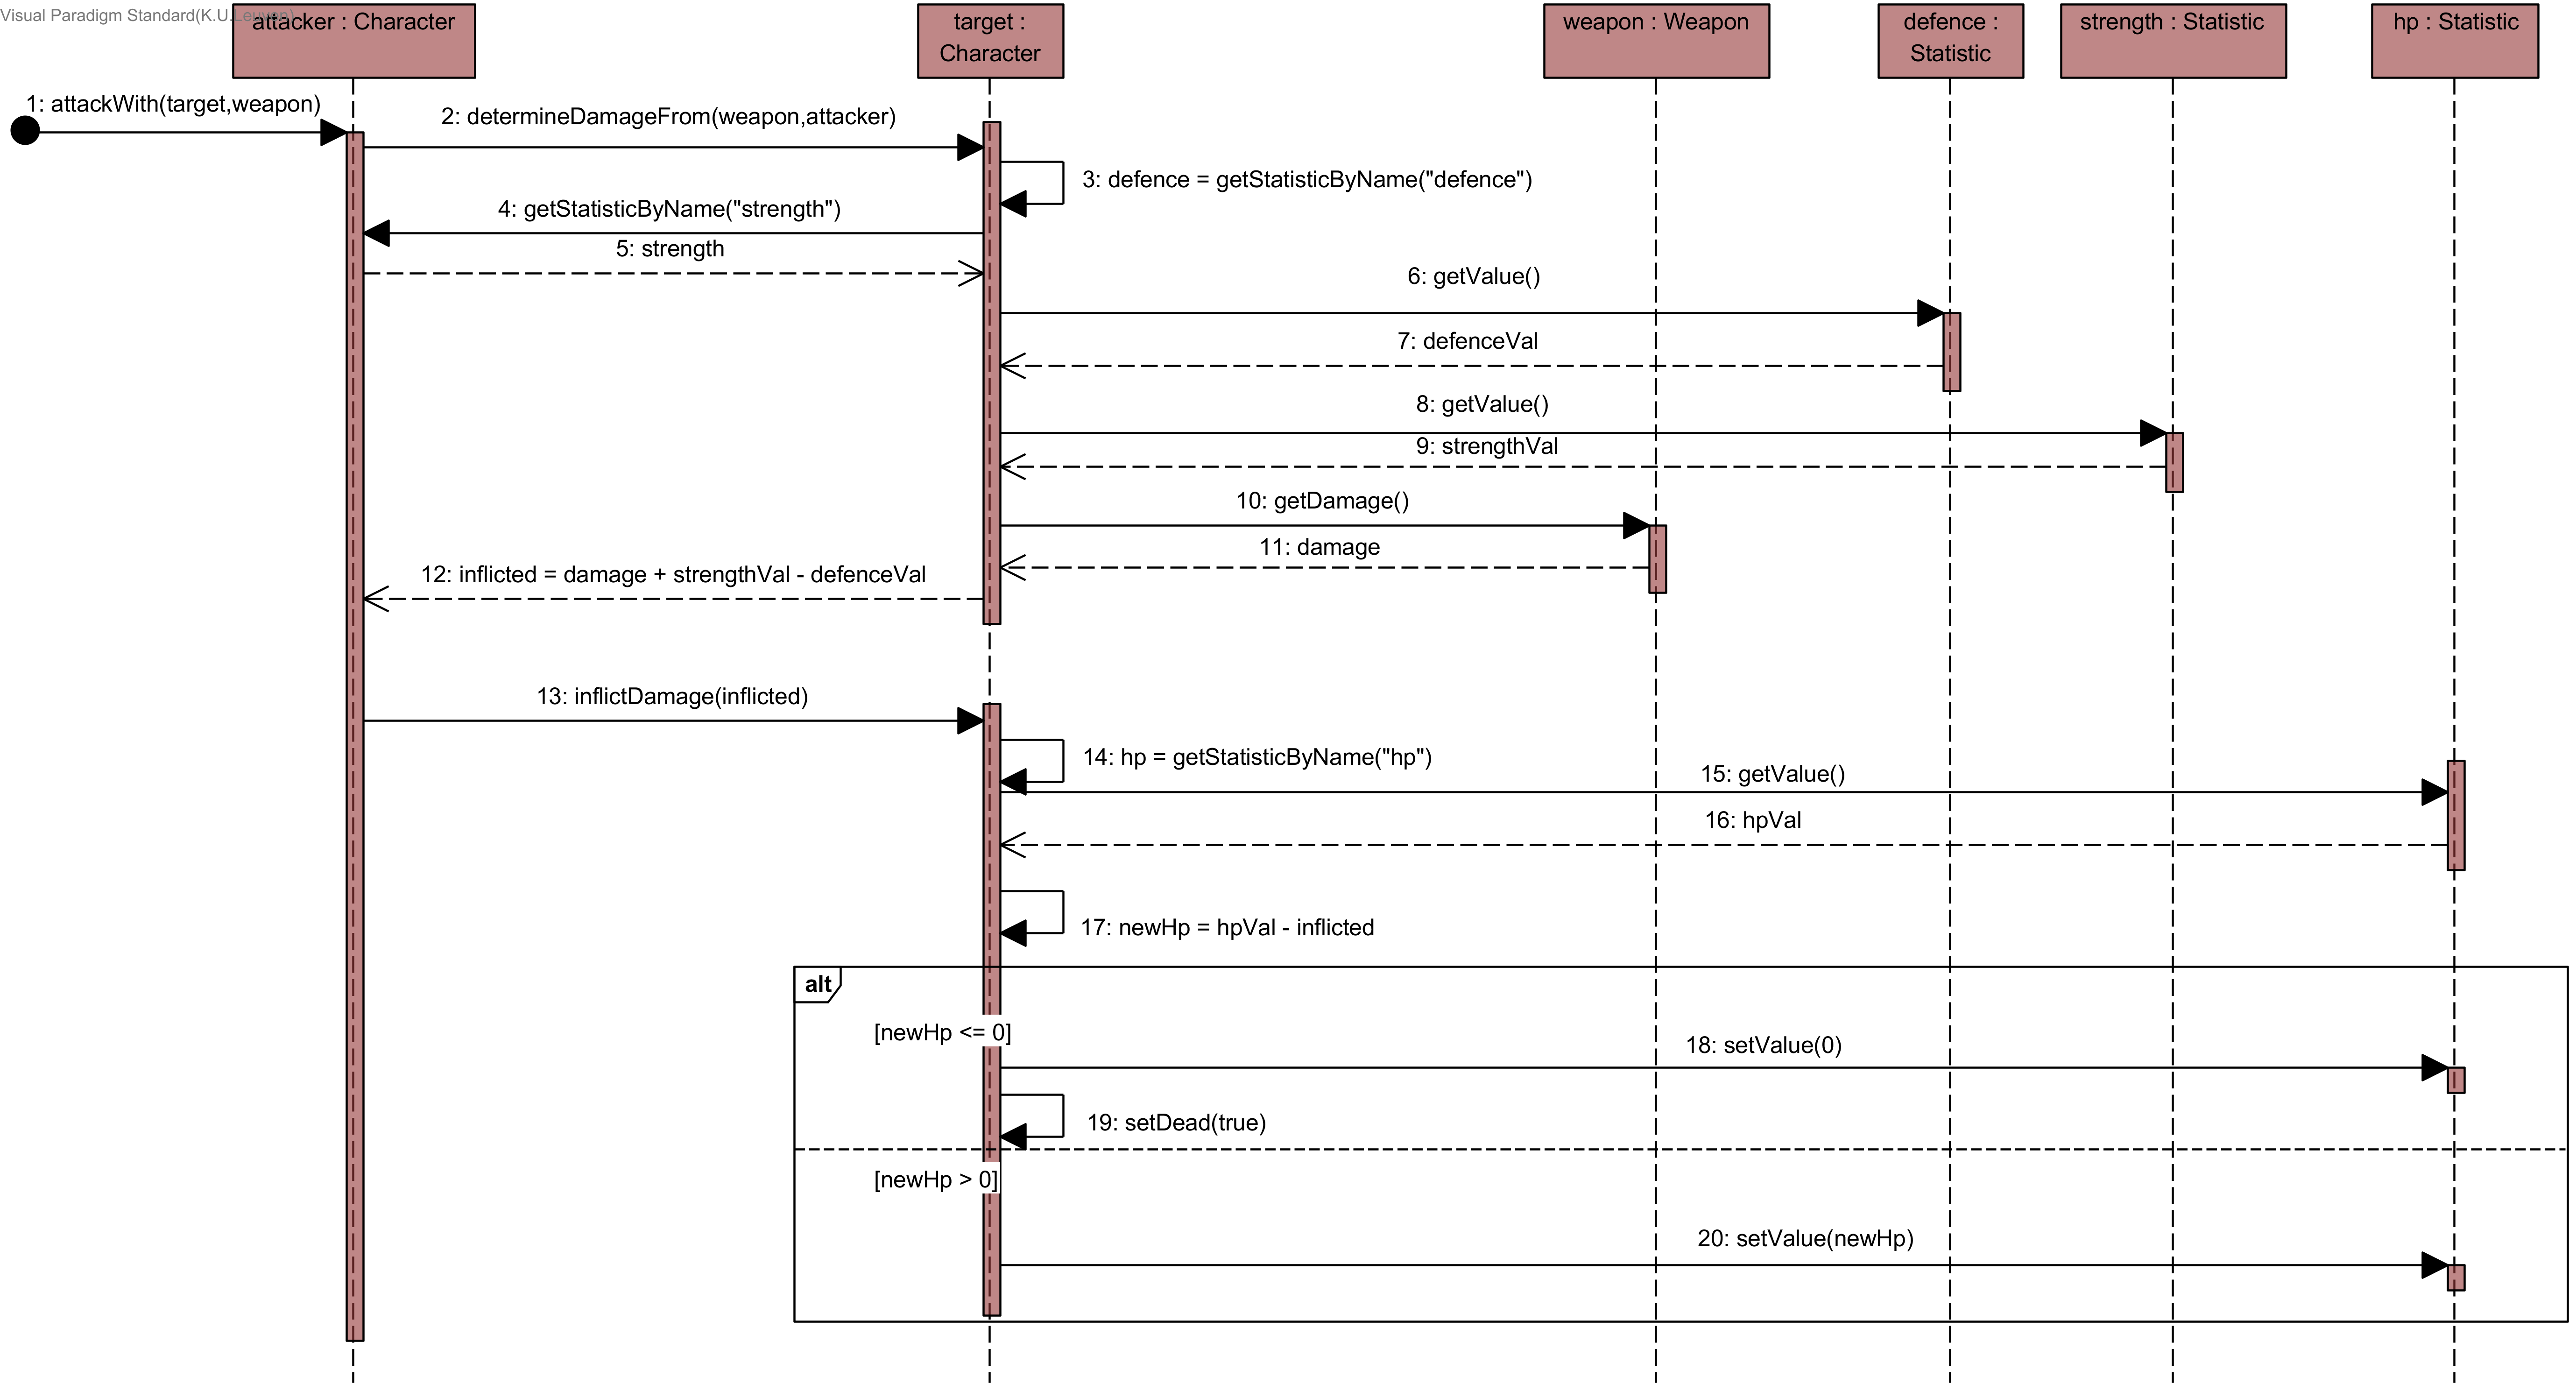
\includegraphics[width=1.5\textwidth]{chap-gedrag/seq-diagram-game.png}
	\caption{Sequentiediagram gebaseerd op het klassediagram van figuur \ref{fig:diagram-voorbeeld}}
\end{figure}
\end{landscape}

\subsection{De keuze voor lineaire tijdscalculus}
UML-diagrammen schrijven mogelijke toestanden van, en acties, op softwaresystemen voor. Die systemen kunnen van toestand veranderen tussen tijdstappen. Sequentiediagrammen zijn een manier om te beschrijven hoe zulke veranderingen teweeg kunnen gebracht worden. Tijdens de uitvoering van een sequentiediagram mag het systeem enkel veranderen zoals beschreven door de huidige actie. Daarom hebben we een mechanisme nodig binnen FO(.) dat dynamische systemen en acties op deze kan beschrijven. Tegelijk moet dat mechanisme garanderen dat eigenschappen van het systeem die niet worden be\"invloed door de huidige beschouwde actie van het sequentiediagram niet veranderen. Lineaire tijdscalculus\cite{BogaertsBart2014Sdsu}, oftewel LTC, voldoet aan deze voorwaarden. Daarom zullen we om sequentiediagrammen uitvoerbaar te maken binnen FO(.) het generatieproces voor het vocabularium en de theorie dat we bekomen zijn in hoofdstuk \ref{sec:consistentie} uitbreiden volgens de principes van LTC.

In de volgende secties werken we deze uitbreiding uit voor het sequentiediagram in figuur \ref{fig:seq-diagram-game}.

\subsection{Uitbreiding van het vocabularium}
In LTC is tijd een centraal concept, dus daarom introduceren we allereerst een logisch type $Time \subset \mathbb{N}$. Verder defini\"eren we een parti\"ele functie \textit{Next(Time)} dat voor alle tijdpunten het volgende tijdpunt geeft behalve voor het laatst mogelijke tijdpunt. We defini\"eren ook een constante \textit{Start}, wat het eerst mogelijke tijdpunt aanduidt.

Voor elk tijdpunt is het mogelijk dat er een bepaalde instructie van het sequentiediagram wordt uitgevoerd. We duiden deze instructie aan met zijn volgnummer.
Deze volgnummers gebruiken we als instructieteller, en daarvoor defini\"eren we een logisch type $SDPoint \subset \mathbb{N}$.

Om te garanderen dat de instructievolgorde opgelegd door het sequentiediagram gevolgd wordt, maken we deze instructieteller inertieel en introduceren we deze symbolen:

\begin{itemize}
	\item Het toestandspredicaat: \textit{SDPointAt(Time, SDPoint)}
	\item Het begintoestandspredicaat: \textit{I\_SDPointAt(SDPoint)}
	\item Het causatiepredicaat: \textit{C\_SDPointAt(Time, SDPoint)}
\end{itemize}

We moeten ook de instanties waarop gehandeld wordt in het sequentiediagram kunnen benoemen. Om te garanderen dat de instanties die vernoemd worden altijd verwijzen naar hetzelfde object, maken we ook de instanties inertieel. Voor \textit{attacker} verkrijgen we dan bijvoorbeeld:

\begin{itemize}
	\item \textit{AttackerT(Time, Character)}
	\item \textit{I\_AttackerT(Character)}
	\item \textit{C\_AttackerT(Time, Character)}
\end{itemize}

Het is ook mogelijk dat in een instructie een variabele intern aan het sequentiediagram wordt gedefinieerd. Zo is er instructie 7 waar een return-instructie \textit{defenceVal} definieert en ook instructie 12 die de waarde van \textit{inflicted} definieert als een som van andere variabelen. Deze variabelen willen we ook kunnen benoemen en maken we inertieel. Voor alle zulke variabelen defini\"eren we ook predicaten zoals hierboven voor \textit{attacker}.

We passen ook de predicaten die overeenkomen met klasseattributen aan. Het kan immers zijn dat de waarde van een attribuut wordt aangepast, zoals in instructie 18 die de waarde van \textit{value} van object \textit{hp} van klasse \textit{Statistic} verandert naar 0. Klasseattributen maken we ook inertieel. Voor \textit{value} in \textit{Statistic} krijgen we dan:

\begin{itemize}
	\item \textit{Statisticvalue(Time, Statistic, LimitedInt)}
	\item \textit{I\_Statisticvalue(Statistic, LimitedInt)}
	\item \textit{C\_Statisticvalue(Time, Statistic, LimitedInt)}
	\item En het oncausatiepredicaat: \textit{Cn\_Statisticvalue(Time, Statistic, LimitedInt)}
\end{itemize}

Hier voegen we een oncausatiepredicaat toe omdat het mogelijk is dat een attribuut meer dan \'e\'en waarde heeft op een bepaald tijdstip. Met dit predicaat geven we aan dat bepaalde waardes die voor een bepaalde tijdstap gelden ongedaan moeten worden gemaakt in de volgende tijdstap.

\subsection{Uitbreiden van de theorie}
Voor elke inerti\"ele eigenschap van het systeem moeten er twee dingen gebeuren: Toestandszinnen opstellen en voorwaardes voor causatiezinnen en oncausatiezinnen specificeren. Het resultaat is een inductieve definitie die de inerti\"ele predicaten definieert en een inductieve definitie die de causatiepredicaten en oncausatiepredicaten definieert.

\subsubsection{Toestandszinnen opstellen}
Toestandszinnen worden geschreven in termen van begintoestandspredicaten, causatiepredicaten en oncausatiepredicaten. Ze garanderen dat inerti\"ele eigenschappen enkel veranderen wanneer het ook echt de bedoeling is dat ze veranderen.

Als eerste kijken we naar toestandszinnen voor \textit{SDPointAt}. \textit{I\_SDPointAt} geeft aan welke de eerste instructie is die we willen uitvoeren, en daarom schrijven we een definitie die deze overeenkomst uitdrukt:

\begin{align}
	\forall{s}[SDPoint](SDPointAt(Start, s) \leftarrow I\_SDPointAt(s)).
\end{align}


De volgende definities gebruiken het causatiepredicaat:

\begin{align}
	\forall{t}[Time]\forall{s}[SDPoint](SDPointAt(Next(t), s) \leftarrow C\_SDPointAt(Next(t), s)). \label{eq:sdcauses}
\end{align}
\begin{align}
	\forall{t}[Time]\forall{s}[SDPoint](SDPointAt(Next(t), s) \leftarrow SDPointAt(t, s) \nonumber \\ \land{} \space \lnot{}(\exists{s1}[SDPoint](C\_SDPointAt(Next(t), s1)))). \label{eq:sduncauses}
\end{align}

Zin \ref{eq:sdcauses} zorgt ervoor dat de huidige waarde van \textit{SDPointAt} wordt behouden tenzij er een oorzaak is voor verandering.

We schrijven gelijkaardige definities voor de predicaten die overeenkomen met instanties die vernoemd worden in het sequentiediagram (zoals \textit{attacker}).

\parbreak

Voor klasseattributen verloopt dit ook gelijkaardig, maar we wijken af van het formaat van zin \ref{eq:sduncauses} door als volgt het oncausatiepredicaat te gebruiken:

\begin{align*}
	\forall{t}[Time]\forall{s}[Statistic]\forall{i}[LimitedInt](Statisticvalue(Next(t), s, i) \\ \leftarrow Statisticvalue(t, s, i) \land \lnot Cn\_Statisticvalue(Next(t), s, i)).
\end{align*}

\subsubsection{Voorwaardes voor causatie en oncausatie}
We kijken eerst naar klasseattributen. Een aantal ervan worden niet aangepast, wat we bijvoorbeeld neerschrijven voor \textit{range} in \textit{Weapon} als volgt:

\begin{align*}
	\forall{t}[Time]\forall{w}[Weapon]\forall{i}[LimitedInt](C\_Weaponrange(t, w, i) \leftarrow false).
\end{align*}
\begin{align*}
	\forall{t}[Time]\forall{w}[Weapon]\forall{i}[LimitedInt](Cn\_Weaponrange(t, w, i) \leftarrow false).
\end{align*}

Voor de klasseattributen die wel worden aangepast, kijken we naar de instructies die zulke aanpassingen doorvoeren. Voor \textit{value} in \textit{Statistic} zijn dit instructie 18 en 20. We kijken eerst naar de causatiezin en oncausatiezin die volgen uit instructie 18:

\begin{align*}
	\forall{t}[Time]\forall{s}[Statistic](C\_Statisticvalue(t, s, 0) \leftarrow SDPointAt(t, 18) \land HpT(t, s).
\end{align*}
\begin{align*}
	\forall{t}[Time]\forall{s}[Statistic]\forall{i}[LimitedInt](Cn\_Statisticvalue(Next(t), s, v) \\ \leftarrow SDPointAt(Next(t), 18) \land HpT(t, s) \land Statisticvalue(t, s, i) \land \lnot{}(i = 0).
\end{align*}

Aangezien in instructie 18 de instantie \textit{hp} wordt aangesproken, gebruiken we \textit{HpT} om te verzekeren dat de waarde van het juiste logisch object wordt veranderd. \textit{value} kan ook maar \'e\'en waarde tegelijk hebben, en daarom schrijven we een oncausatiezin om te verzekeren dat de vorige waarde wordt gewist.

Kijken we nu naar de definities die voortvloeien uit instructie 20:

\begin{align*}
	&\forall{t}[Time]\forall{s}[Statistic]\forall{i}[LimitedInt](C\_Statisticvalue(t, s, i) \\ &\leftarrow SDPointAt(t, 20) \land HpT(t, s) \land NewHpT(t, i)).
\end{align*}
\begin{align*}
&\forall{t}[Time]\forall{s}[Statistic]\forall{i}[LimitedInt](Cn\_Statisticvalue(Next(t), s, i) \\ &\leftarrow SDPointAt(Next(t), 20) \land HpT(t, s) \land Statisticvalue(t, s, i) \land \lnot{}NewHpT(Next(t), i)).
\end{align*}

Het verschil hier is dat we \textit{NewHpT} erbij betrekken omdat we de waarde van \textit{hp} veranderen naar de waarde van \textit{newHp} in plaats van het te veranderen naar 0.

\parbreak

Het volgende waar we naar kijken zijn de causatiezinnen voor \textit{SDPointAt}. Wat we hier willen uitdrukken is dat normaal gezien tussen instructies de instructieteller telkens met \'e\'en wordt verhoogd, tenzij een grens van een \textit{if-else}-constructie of een lus is bereikt. In dat geval kan het zijn dat de instructieteller verspringt afhankelijk van de voorwaarde die vernoemd wordt voor zulke constructies.

Voor deze sequentiediagram krijgen we:

\begin{align}
	&\forall{t}[Time]\forall{s}[SDPoint](C\_SDPointAt(Next(t), (s+1) \leftarrow SDPointAt(t, s) \nonumber \\ &\land \lnot{}((s = 17) \lor (s = 19))). \label{eq:sdprog} \\
	&\forall{t}[Time](C\_SDPointAt(Next(t), 18) \leftarrow SDPointAt(t, 17) \land \nonumber \\ &(\exists{i}[LimitedInt](NewHpT(t, i) \land i <= 0))). \label{eq:sdif} \\
	&\forall{t}[Time](C\_SDPointAt(Next(t), 20) \leftarrow SDPointAt(t, 17 ) \land \nonumber \\ &(\exists{i}[LimitedInt](NewHpT(t, i) \land i > 0))). \label{eq:sdthen} \\
	&\forall{t}[Time](C\_SDPointAt(Next(t), 21) \leftarrow SDPointAt(t, 19) \lor SDPointAt(t, 20)). \label{eq:sdexit}
\end{align}

Zin \ref{eq:sdprog} verzekert het juiste gedrag van instructieteller, namelijk dat hij doorgaans met \'e\'en wordt verhoogd tussen tijdstappen. De uitzonderingen worden hier ook opgelijst; in dit geval verspringt de teller wanneer men het begin van de \textit{if-else}-constructie tegenkomt en wanneer het einde van het \textit{if}-deel is bereikt. Zinnen \ref{eq:sdif} en \ref{eq:sdthen} controleren de voorwaarde voor de uitvoering van het \textit{if}- en \textit{else}-deel en selecteren wat correct is. Zin \ref{eq:sdexit} zegt dat zowel het \textit{if}-deel als het \textit{else}-deel uitkomen op de instructie die direct volgt op de \textit{if-else}-constructie.

\parbreak

Als laatste zijn er de causatiezinnen voor de verscheidene variabelen die worden aangemaakt en aangesproken in het sequentiediagram. Een aantal van deze variabelen veranderen niet doorheen de uitvoering van het sequentiediagram en er wordt verondersteld dat deze al bekend zijn v\'o\'or de uitvoering begint. Deze variabelen zijn diegenen die betrokken zijn bij de eerste instructie: \textit{attacker}, de instantie die de eerste oproep ontvangt, en \textit{target} en \textit{weapon}, die als parameter worden opgegeven.

Voor de andere variabelen wordt er een causatiezin toegevoegd voor elke instructie die een waarde toekent aan die variabele. Als voorbeeld bekijken we instructie 3:

\begin{align*}
	&\forall{t}[Time]\forall{d}[Statistic](C\_DefenceT(t, d) \leftarrow SDPointAt(t, 3) \land \exists{c}[Character](TargetT(t, c) \\ &\land CharacterandStatistic(c, d) \land Statisticname(t, d, "defence"))).
\end{align*}


De zin drukt uit dat de getter wordt opgeroepen op \textit{target} en dat er wordt gevraagd naar een instantie van \textit{Statistic} dat in verband staat met \textit{target} en als naam "defence" heeft. Die instantie wordt dan als waarde toegekend aan de variabele \textit{defence}.

Zie appendix \ref{app:seq-diagram-game} voor het volledig model voor het gedrag van het sequentiediagram in figuur \ref{fig:seq-diagram-game}.


\subsection{Interactie tussen meerdere sequentiediagrammen}